%%%%%%%%%%%%%%%%%%%%%%%%%%%%%%%%%%%%%%%%%%%%%%%%%%%%%%%%%%%%%%%%%%%%%%
% Overleaf (WriteLaTeX) Example: Molecular Chemistry Presentation
%
% Source: http://www.overleaf.com
%
% In these slides we show how Overleaf can be used with standard 
% chemistry packages to easily create professional presentations.
% 
% Feel free to distribute this example, but please keep the referral
% to overleaf.com
% 
%%%%%%%%%%%%%%%%%%%%%%%%%%%%%%%%%%%%%%%%%%%%%%%%%%%%%%%%%%%%%%%%%%%%%%

\documentclass{beamer}

\mode<presentation>
{
  \usetheme{Madrid}       % or try default, Darmstadt, Warsaw, ...
  \usecolortheme{default} % or try albatross, beaver, crane, ...
  \usefonttheme{default}    % or try default, structurebold, ...
  \setbeamertemplate{navigation symbols}{}
  \setbeamertemplate{caption}[numbered]
} 

\usepackage[english]{babel}
\usepackage[utf8x]{inputenc}
\usepackage{chemfig}
\usepackage[version=3]{mhchem}

\usepackage{hyperref}
  \hypersetup{colorlinks=true}
  \hypersetup{urlcolor=blue}
  \hypersetup{linkcolor = .}
\usepackage{xcolor}
\usepackage{siunitx}
  \sisetup{separate-uncertainty = true}
\usepackage{physics}
\usepackage[font=small,labelfont=bf]{caption}
\usepackage{subcaption}
\usepackage[en-GB]{datetime2}
\usepackage{feynmp}
\DeclareGraphicsRule{*}{mps}{*}{}

\usepackage{scalerel}
\newcommand{\mylbrace}[2]{\vspace{#2pt}\hspace{6pt}\scaleleftright[\dimexpr5pt+#1\dimexpr0.06pt]{\lbrace}{\rule[\dimexpr2pt-#1\dimexpr0.5pt]{-4pt}{#1pt}}{.}}
\newcommand{\myrbrace}[2]{\vspace{#2pt}\scaleleftright[\dimexpr5pt+#1\dimexpr0.06pt]{.}{\rule[\dimexpr2pt-#1\dimexpr0.5pt]{-4pt}{#1pt}}{\rbrace}\hspace{6pt}}

% Here's where the presentation starts, with the info for the title slide
\title[BESIII Oxford]{BESIII Oxford Group Meeting}
\author{Martin Tat}
\institute{Oxford LHCb}
\date{25th February 2021}

\titlegraphic{
\includegraphics[width = 5cm, height = 3.8cm]{lhcb.jpg}\hspace{1cm}~%
              
\includegraphics[width = 5cm, height = 3.8cm]{bes3.png}}

\begin{document}

\begin{frame}
  \titlepage
\end{frame}

% These three lines create an automatically generated table of contents.
%\begin{frame}{Outline}
%  \tableofcontents
%\end{frame}

\section{Intorduction, double tags}
\begin{frame}{Introduction}
  \begin{itemize}
    \item{Double tagged $D\to K^+K^-\pi^+\pi^-$ events}
    \item{Previously: $KK$, $K\pi$, $K\pi\pi^0$, $K_S\pi^0$ tags}
    \item{Current progress: Have now implemented the following tags:}
    \item{CP tags:}
    \begin{itemize}
      \item{$KK$, $\pi\pi$, $K_S\pi^0$, $K_S\pi^0\pi^0$, $\pi\pi\pi^0$, $K_S\eta$, $K_S\eta'(\pi\pi\eta)$, $K_S\eta'(\rho\gamma)$, $K_S(\eta, \omega)(\pi\pi\pi^0)$, $K_S\phi$}
    \end{itemize}
    \item{CP conjugate tags:}
    \begin{itemize}
      \item{$K_S\pi\pi$, $KK\pi\pi$}
    \end{itemize}
    \item{Flavour tags:}
    \begin{itemize}
      \item{$K\pi$, $K\pi\pi^0$}
    \end{itemize}
    \item{Ran over full $2010$ and $2011$ MC $D^0\bar{D}^0$ sample ($20x$ luminosity)}
  \end{itemize}
\end{frame}

\section{Selection procedure}
\begin{frame}{Selection procedure}
  \begin{itemize}
    \item{Standard cuts in the DTagTool package}
    \item{$\pi^0\to\gamma\gamma$ with $\SI{0.110}{\giga\eV} < m(\gamma\gamma) < \SI{0.155}{\giga\eV}$}
    \item{$\eta\to\gamma\gamma$ with $\SI{0.480}{\giga\eV} < m(\gamma\gamma) < \SI{0.580}{\giga\eV}$}
    \item{$K_S\to\pi\pi$, flight significance cut at $2$}
    \item{All $\pi\pi$ combinations have a flight significance cut at $2$}
    \item{$\phi\to KK$, with $\abs{m(KK) - m_{\text{PDG}}(\phi)} < \SI{0.020}{\giga\eV}$}
    \item{$\eta'\to\pi\pi\eta$, with $\SI{0.940}{\giga\eV} < m(\pi\pi\eta) < \SI{0.976}{\giga\eV}$}
    \item{$\eta'\to\pi\pi\gamma$, with $\SI{0.940}{\giga\eV} < m(\pi\pi\gamma) < \SI{0.970}{\giga\eV}$}
    \item{$\eta\to\pi\pi\pi^0$, with $\SI{0.530}{\giga\eV} < m(\pi\pi\pi^0) < \SI{0.565}{\giga\eV}$}
    \item{$\omega\to\pi\pi\pi^0$, with $\SI{0.750}{\giga\eV} < m(\pi\pi\pi^0) < \SI{0.820}{\giga\eV}$}
  \end{itemize}
\end{frame}

\begin{frame}{Cut on $\Delta E$}
  \begin{itemize}
    \item{Fit double Gaussian and 2nd order polynomial to $\Delta E$}
    \item{Cut at $(-3\sigma, +3\sigma)$ for modes without $\pi^0$}
    \item{Cut at $(-4\sigma, +3\sigma)$ for modes with $\pi^0$ (what about $\eta$?)}
    \item{Fit both signal and tag side}
  \end{itemize}
\end{frame}

\section{$\Delta E$ cut}
\begin{frame}{$\Delta E$ cut on $K\pi$ mode}
  \begin{figure}
    \centering
    \begin{subfigure}{0.5\textwidth}
      \centering
      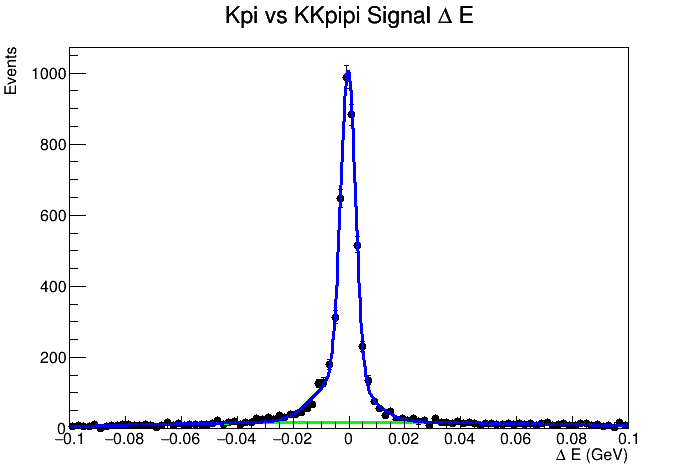
\includegraphics[width=\textwidth]{KpiSignalDeltaE.png}
      \caption{$\Delta E$, $KK\pi\pi$}
    \end{subfigure}%
    \begin{subfigure}{0.5\textwidth}
      \centering
      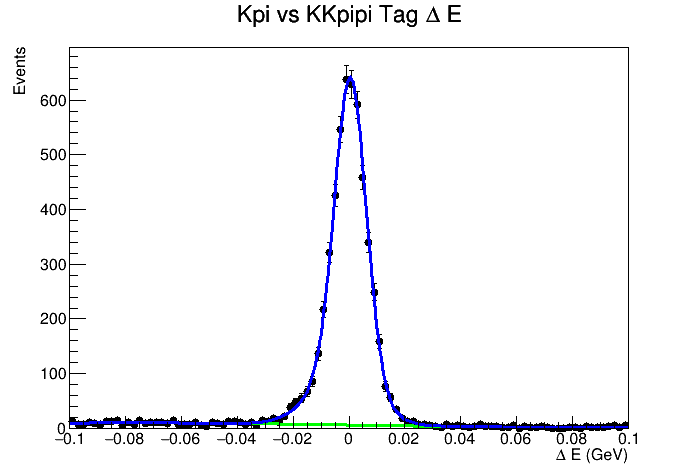
\includegraphics[width=\textwidth]{KpiTagDeltaE.png}
      \caption{$\Delta E$, $K\pi$}
    \end{subfigure}
  \end{figure}
\end{frame}

\begin{frame}{$\Delta E$ cut on $\pi\pi\pi^0$ mode}
  \begin{figure}
    \centering
    \begin{subfigure}{0.5\textwidth}
      \centering
      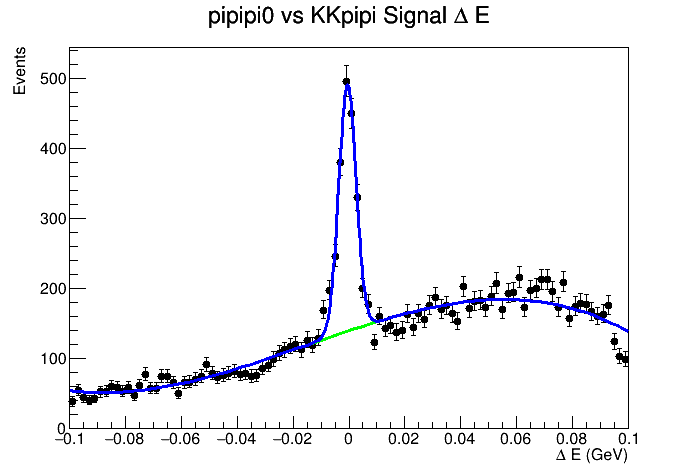
\includegraphics[width=\textwidth]{pipipi0SignalDeltaE.png}
      \caption{$\Delta E$, $KK\pi\pi$}
    \end{subfigure}%
    \begin{subfigure}{0.5\textwidth}
      \centering
      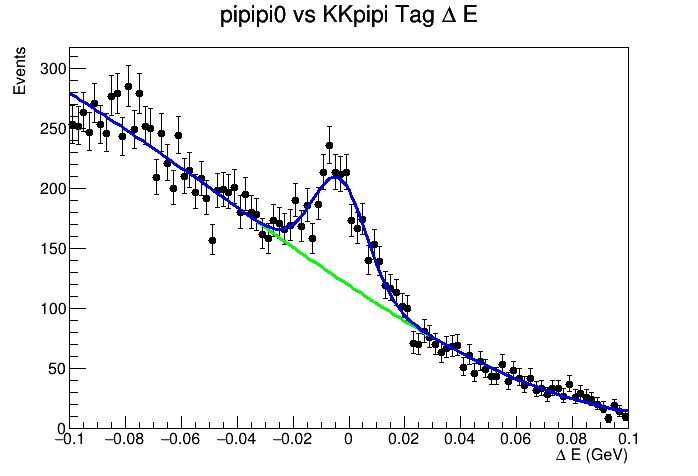
\includegraphics[width=\textwidth]{pipipi0TagDeltaE.png}
      \caption{$\Delta E$, $\pi\pi\pi^0$}
    \end{subfigure}
  \end{figure}
\end{frame}

\begin{frame}{$\Delta E$ cut on $K_S\eta'(\pi\pi\gamma)$ mode}
  \begin{figure}
    \centering
    \begin{subfigure}{0.5\textwidth}
      \centering
      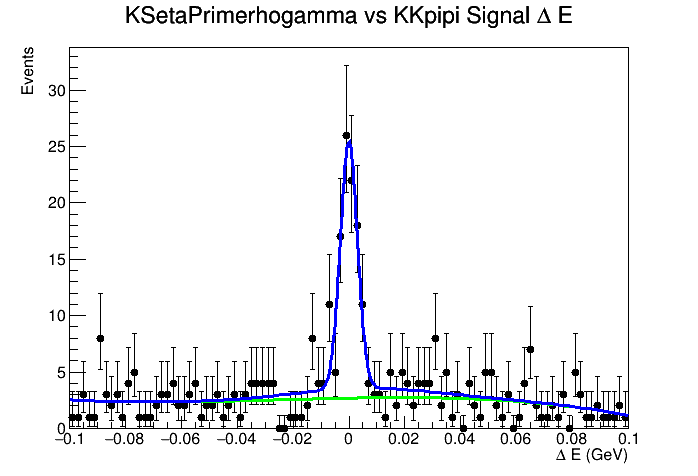
\includegraphics[width=\textwidth]{KSetaPrimerhogammaSignalDeltaE.png}
      \caption{$\Delta E$, $KK\pi\pi$}
    \end{subfigure}%
    \begin{subfigure}{0.5\textwidth}
      \centering
      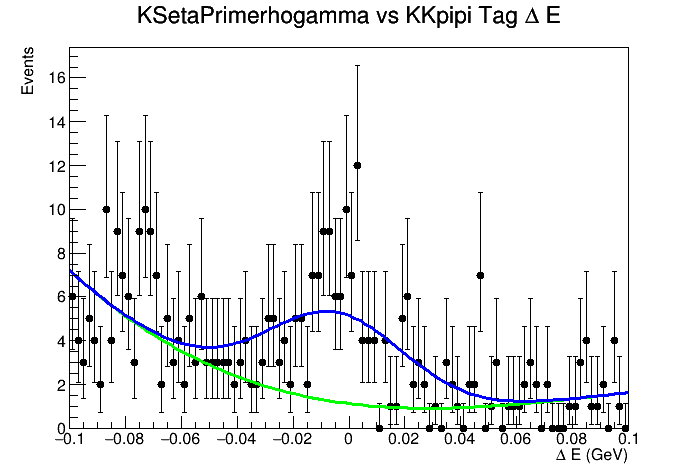
\includegraphics[width=\textwidth]{KSetaPrimerhogammaTagDeltaE.png}
      \caption{$\Delta E$, $K_S\eta'(\pi\pi\gamma)$}
    \end{subfigure}
  \end{figure}
\end{frame}

\begin{frame}{$\Delta E$ cut on other modes}
  \begin{figure}
    \centering
    \begin{subfigure}{0.4\textwidth}
      \centering
      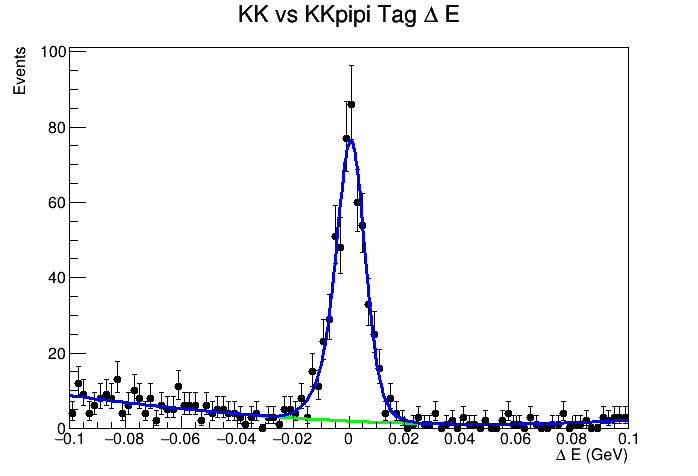
\includegraphics[width=\textwidth]{KKTagDeltaE.png}
      \caption{$\Delta E$, $KK$}
    \end{subfigure}%
    \begin{subfigure}{0.4\textwidth}
      \centering
      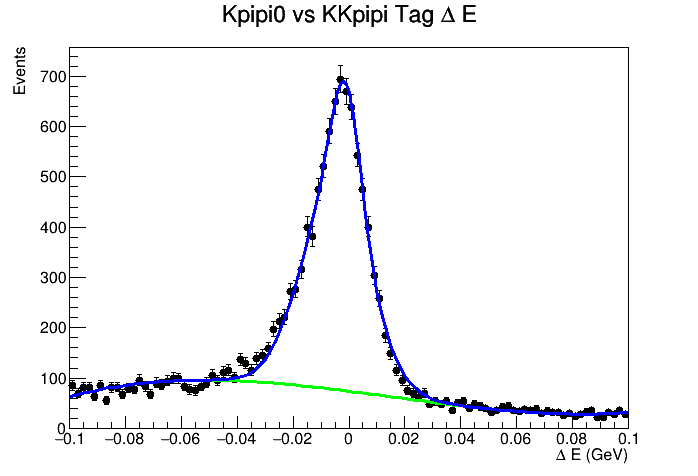
\includegraphics[width=\textwidth]{Kpipi0TagDeltaE.png}
      \caption{$\Delta E$, $K\pi\pi^0$}
    \end{subfigure}
    \centering
    \begin{subfigure}{0.4\textwidth}
      \centering
      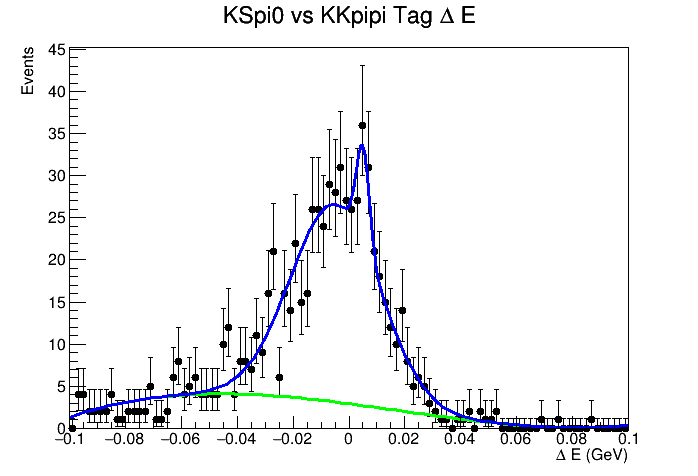
\includegraphics[width=\textwidth]{KSpi0TagDeltaE.png}
      \caption{$\Delta E$, $K_S\pi^0$}
    \end{subfigure}%
    \begin{subfigure}{0.4\textwidth}
      \centering
      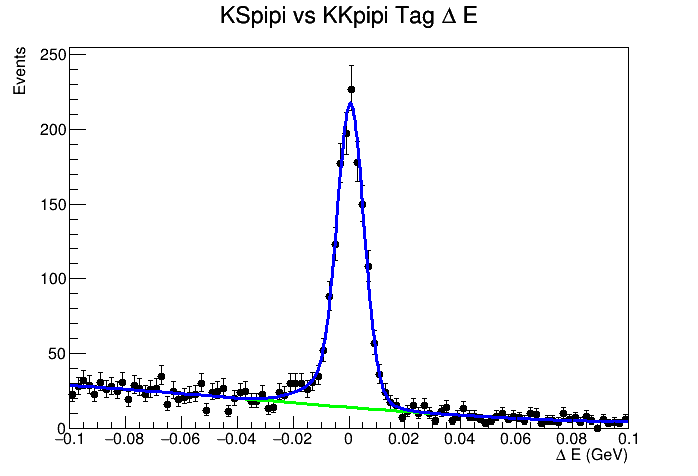
\includegraphics[width=\textwidth]{KSpipiTagDeltaE.png}
      \caption{$\Delta E$, $K_S\pi\pi$}
    \end{subfigure}
  \end{figure}
\end{frame}

\begin{frame}{$\Delta E$ cut on other modes}
  \begin{figure}
    \centering
    \begin{subfigure}{0.4\textwidth}
      \centering
      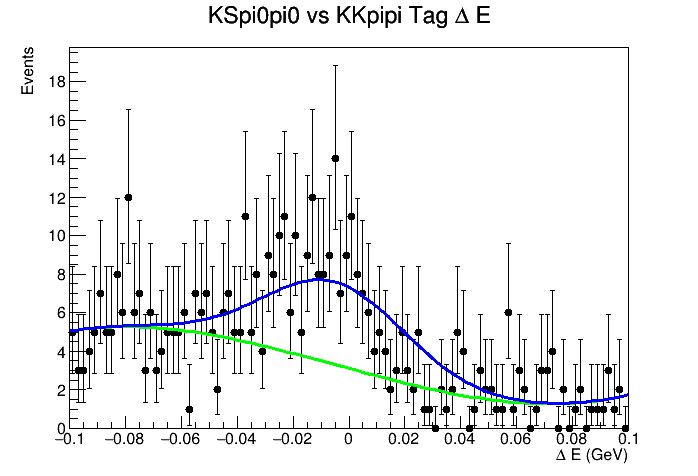
\includegraphics[width=\textwidth]{KSpi0pi0TagDeltaE.png}
      \caption{$\Delta E$, $K_S\pi^0\pi^0$}
    \end{subfigure}%
    \begin{subfigure}{0.4\textwidth}
      \centering
      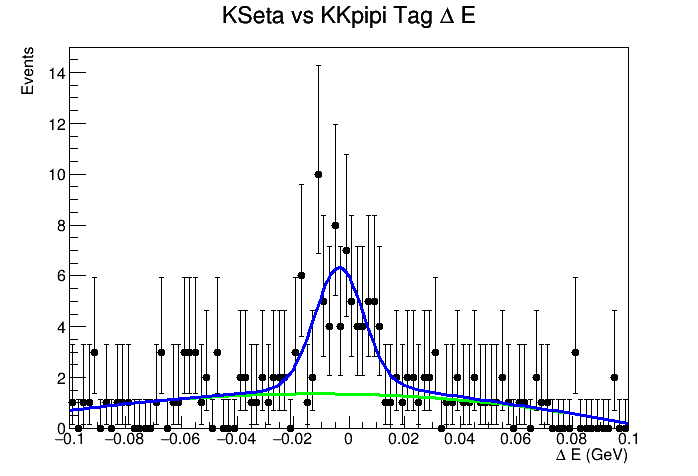
\includegraphics[width=\textwidth]{KSetaTagDeltaE.png}
      \caption{$\Delta E$, $K_S\eta$}
    \end{subfigure}
    \centering
    \begin{subfigure}{0.4\textwidth}
      \centering
      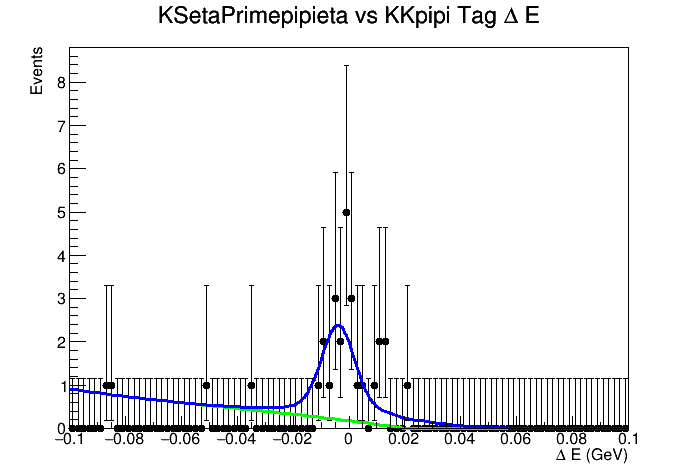
\includegraphics[width=\textwidth]{KSetaPrimepipietaTagDeltaE.png}
      \caption{$\Delta E$, $K_S\eta'(\pi\pi\eta)$}
    \end{subfigure}%
    \begin{subfigure}{0.4\textwidth}
      \centering
      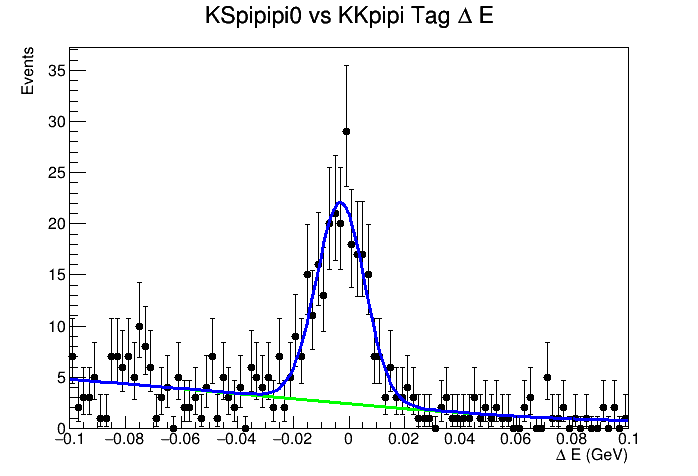
\includegraphics[width=\textwidth]{KSpipipi0TagDeltaE.png}
      \caption{$\Delta E$, $K_S(\eta, \omega)(\pi\pi\pi^0)$}
    \end{subfigure}
  \end{figure}
\end{frame}

\begin{frame}{$\Delta E$ cut on other modes}
  \begin{figure}
    \centering
    \begin{subfigure}{0.4\textwidth}
      \centering
      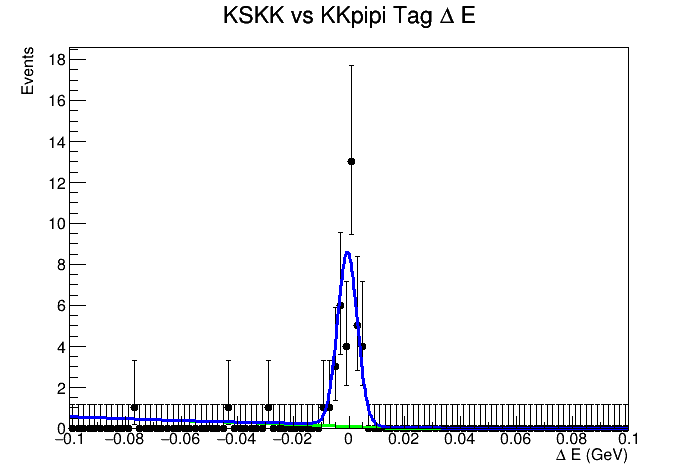
\includegraphics[width=\textwidth]{KSKKTagDeltaE.png}
      \caption{$\Delta E$, $K_SKK$}
    \end{subfigure}%
    \begin{subfigure}{0.4\textwidth}
      \centering
      \includegraphics[width=\textwidth]{KkpipiTagDeltaE.png}
      \caption{$\Delta E$, $KK\pi\pi$}
    \end{subfigure}
    \centering
    \begin{subfigure}{0.4\textwidth}
      \centering
      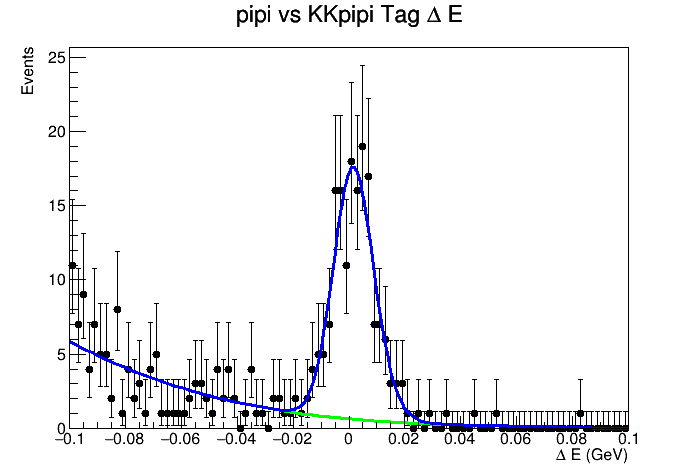
\includegraphics[width=\textwidth]{pipiTagDeltaE.png}
      \caption{$\Delta E$, $\pi\pi$}
    \end{subfigure}
  \end{figure}
\end{frame}

\begin{frame}{$m_\text{BC}$}
  \begin{figure}
    \centering
    \begin{subfigure}{0.5\textwidth}
      \centering
      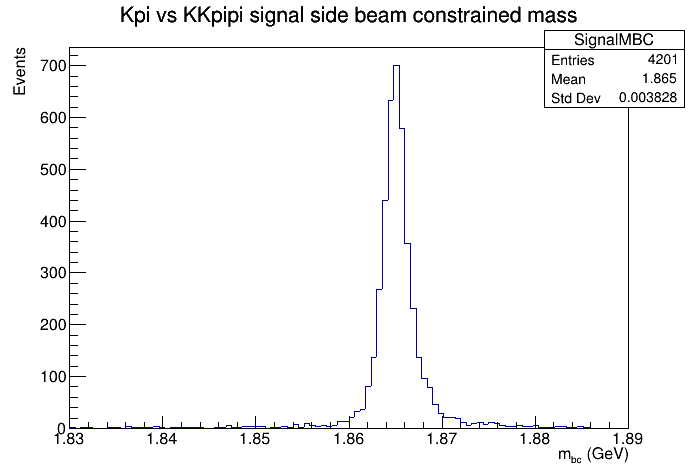
\includegraphics[width=\textwidth]{KpiSignalMBC.png}
      \caption{$m_\text{BC}$, $K\pi$}
    \end{subfigure}%
    \begin{subfigure}{0.5\textwidth}
      \centering
      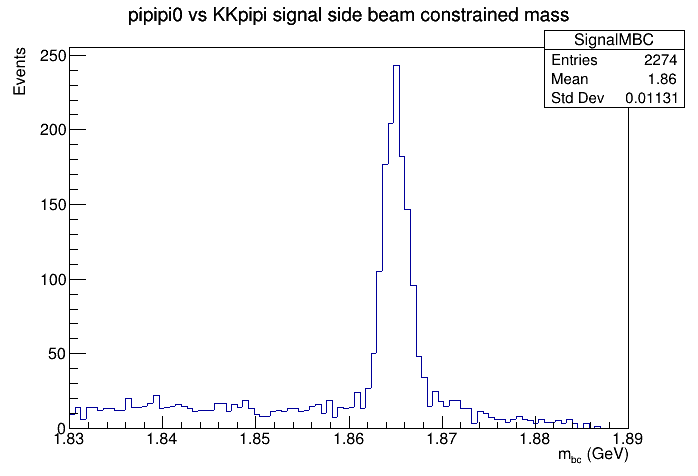
\includegraphics[width=\textwidth]{pipipi0SignalMBC.png}
      \caption{$m_\text{BC}$, $\pi\pi\pi^0$}
    \end{subfigure}
  \end{figure}
\end{frame}

\begin{frame}{$m_\text{BC}$}
  \begin{figure}
    \centering
    \begin{subfigure}{0.4\textwidth}
      \centering
      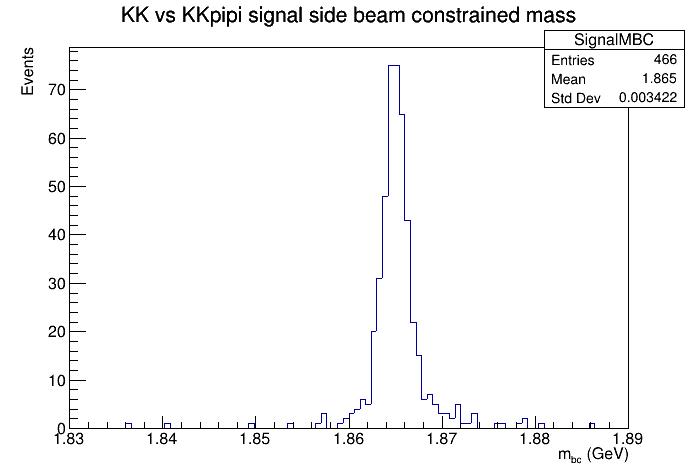
\includegraphics[width=\textwidth]{KKSignalMBC.png}
      \caption{$m_\text{BC}$, $KK$}
    \end{subfigure}%
    \begin{subfigure}{0.4\textwidth}
      \centering
      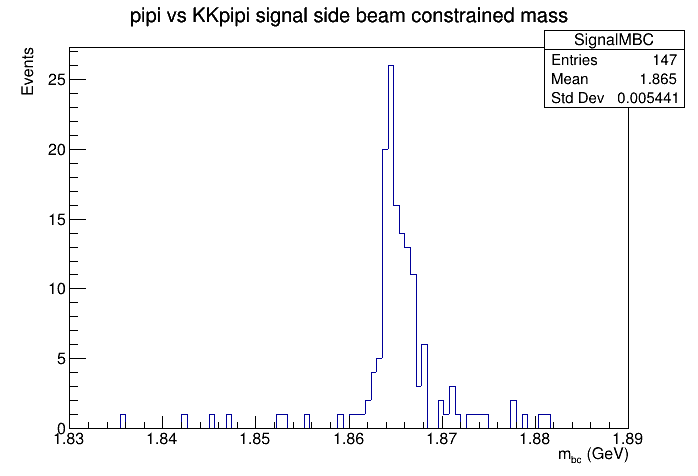
\includegraphics[width=\textwidth]{pipiSignalMBC.png}
      \caption{$m_\text{BC}$, $\pi\pi$}
    \end{subfigure}
    \centering
    \begin{subfigure}{0.4\textwidth}
      \centering
      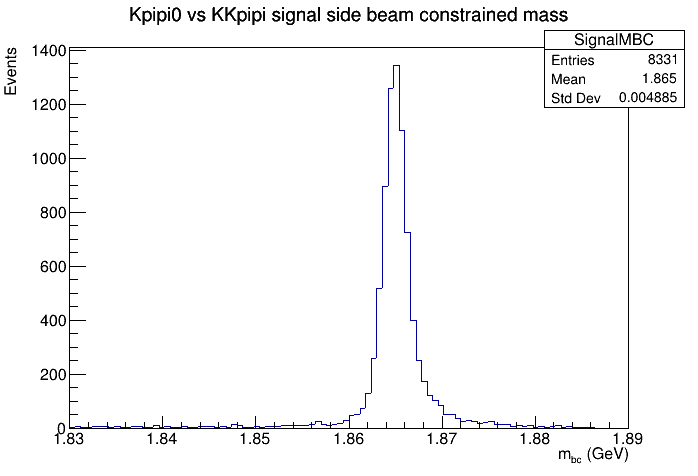
\includegraphics[width=\textwidth]{Kpipi0SignalMBC.png}
      \caption{$m_\text{BC}$, $K\pi\pi^0$}
    \end{subfigure}%
    \begin{subfigure}{0.4\textwidth}
      \centering
      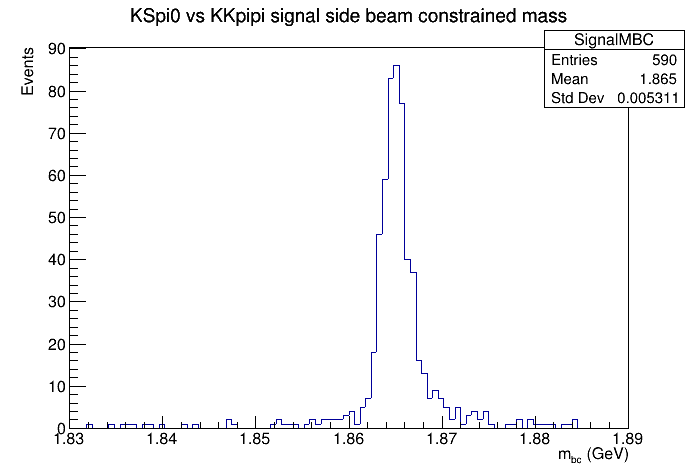
\includegraphics[width=\textwidth]{KSpi0SignalMBC.png}
      \caption{$m_\text{BC}$, $K_S\pi^0$}
    \end{subfigure}
  \end{figure}
\end{frame}

\begin{frame}{$m_\text{BC}$}
  \begin{figure}
    \centering
    \begin{subfigure}{0.4\textwidth}
      \centering
      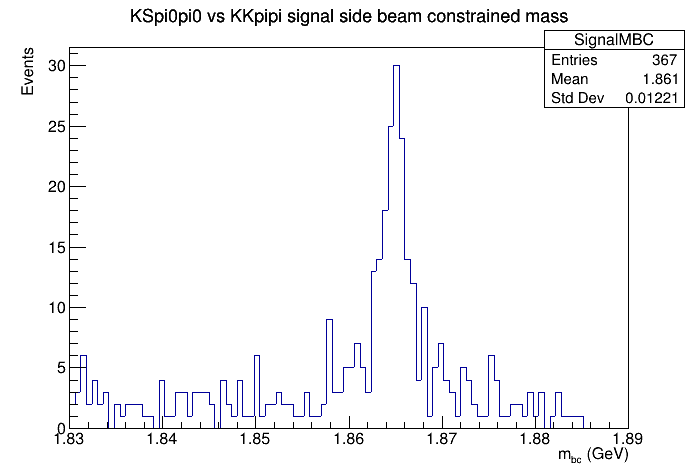
\includegraphics[width=\textwidth]{KSpi0pi0SignalMBC.png}
      \caption{$m_\text{BC}$, $KS\pi^0\pi^0$}
    \end{subfigure}%
    \begin{subfigure}{0.4\textwidth}
      \centering
      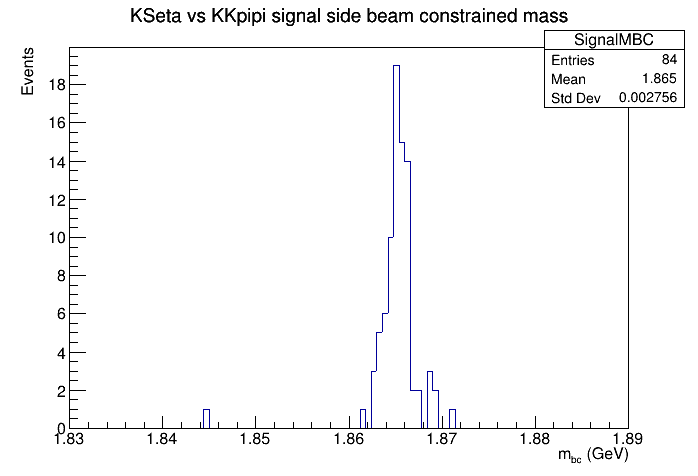
\includegraphics[width=\textwidth]{KSetaSignalMBC.png}
      \caption{$m_\text{BC}$, $K_S\eta$}
    \end{subfigure}
    \centering
    \begin{subfigure}{0.4\textwidth}
      \centering
      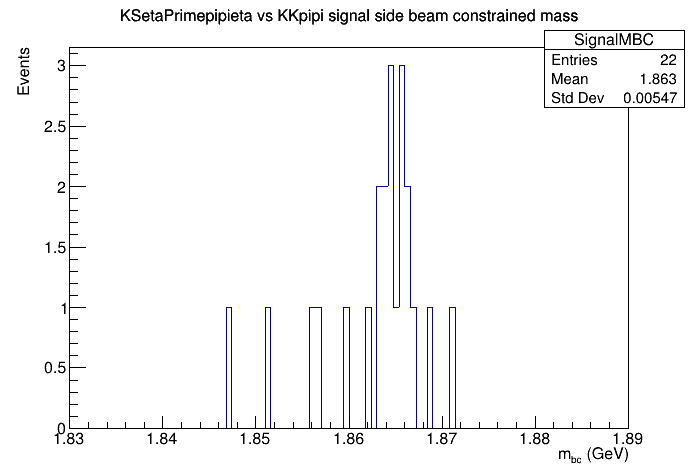
\includegraphics[width=\textwidth]{KSetaPrimepipietaSignalMBC.png}
      \caption{$m_\text{BC}$, $K_S\eta'(\pi\pi\eta)$}
    \end{subfigure}%
    \begin{subfigure}{0.4\textwidth}
      \centering
      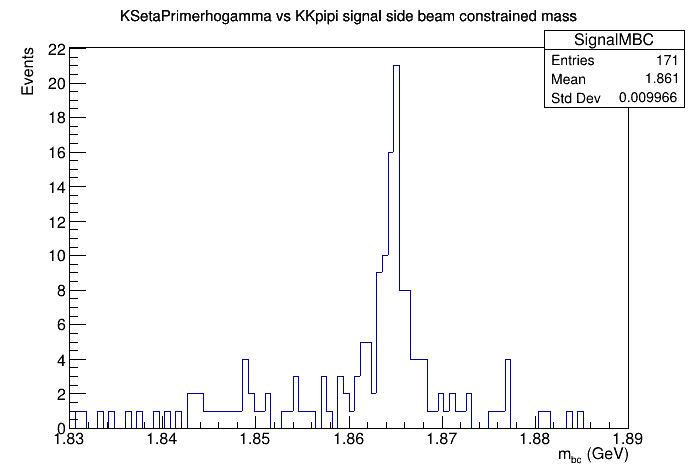
\includegraphics[width=\textwidth]{KSetaPrimerhogammaSignalMBC.png}
      \caption{$m_\text{BC}$, $K_S\eta'(\pi\pi\gamma)$}
    \end{subfigure}
  \end{figure}
\end{frame}

\begin{frame}{$m_\text{BC}$}
  \begin{figure}
    \centering
    \begin{subfigure}{0.4\textwidth}
      \centering
      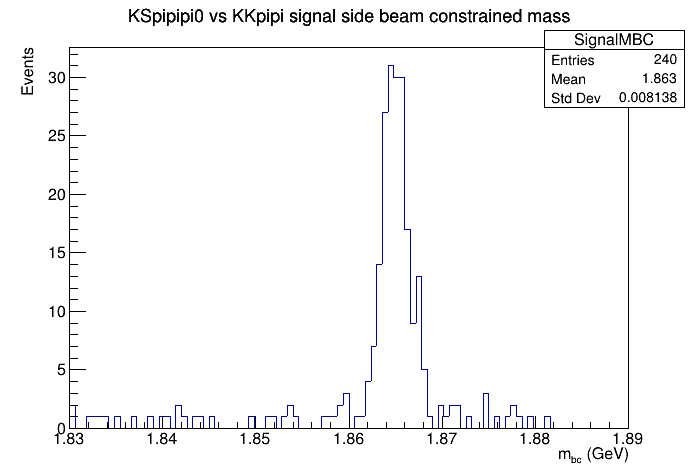
\includegraphics[width=\textwidth]{KSpipipi0SignalMBC.png}
      \caption{$m_\text{BC}$, $K_S(\eta, \omega)(\pi\pi\pi^0)$}
    \end{subfigure}%
    \begin{subfigure}{0.4\textwidth}
      \centering
      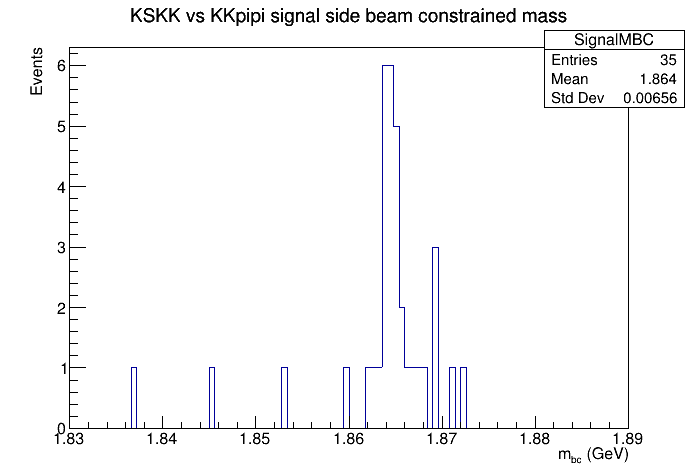
\includegraphics[width=\textwidth]{KSKKSignalMBC.png}
      \caption{$m_\text{BC}$, $K_SKK$}
    \end{subfigure}
    \centering
    \begin{subfigure}{0.4\textwidth}
      \centering
      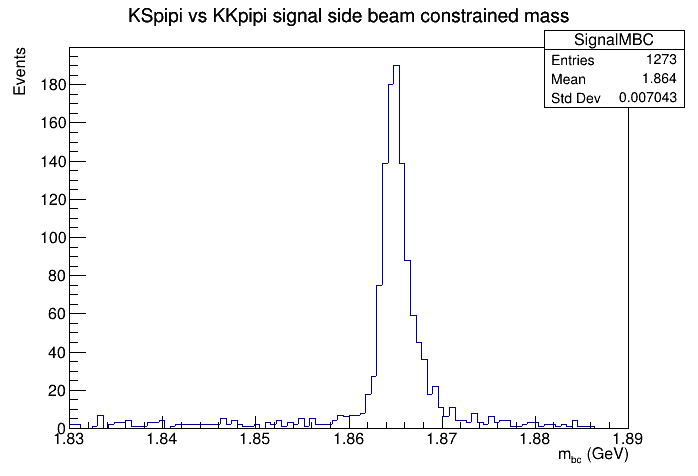
\includegraphics[width=\textwidth]{KSpipiSignalMBC.png}
      \caption{$m_\text{BC}$, $K_S\pi\pi$}
    \end{subfigure}%
    \begin{subfigure}{0.4\textwidth}
      \centering
      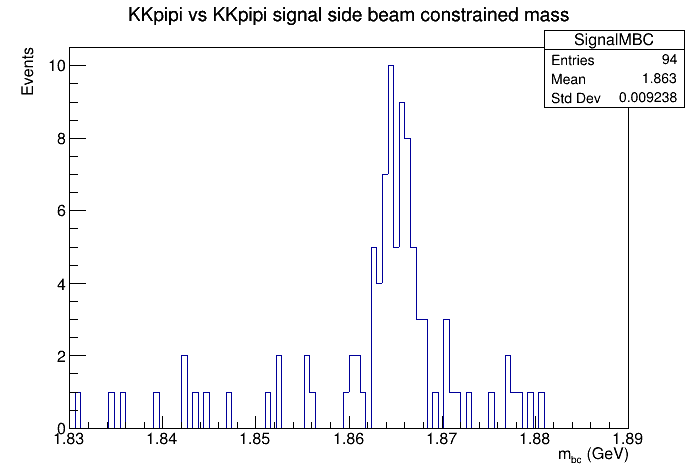
\includegraphics[width=\textwidth]{KKpipiSignalMBC.png}
      \caption{$m_\text{BC}$, $KK\pi\pi$}
    \end{subfigure}
  \end{figure}
\end{frame}

\section{Flat background estimate}
\begin{frame}{Flat background estimate}
  \begin{figure}
    \centering
    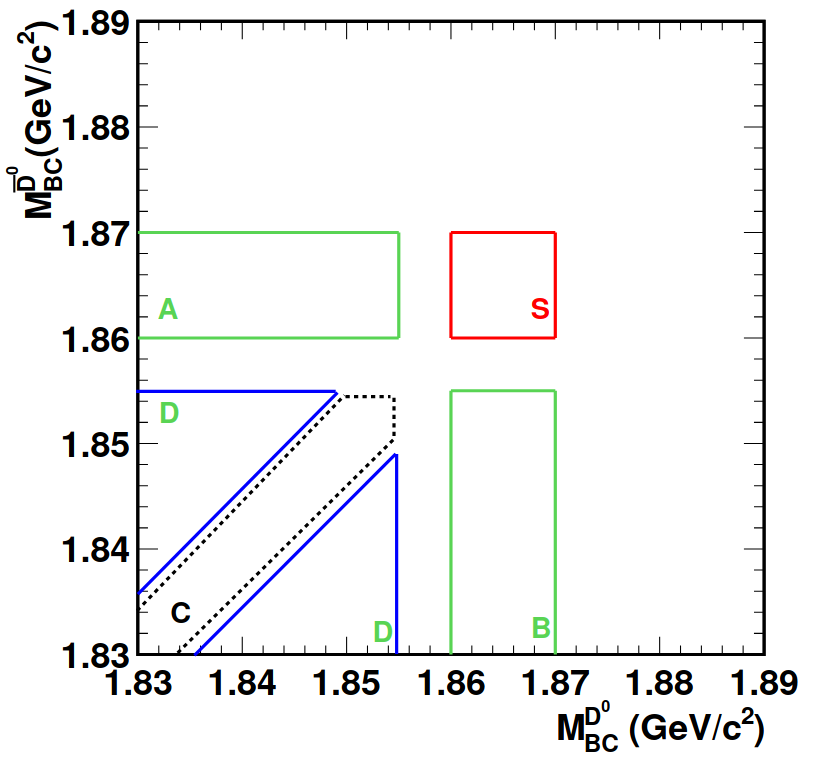
\includegraphics[width=0.5\textwidth]{MBC2D.png}
    \caption{$m_\text{BC}$ plane, BESIII $K_S^0K^+K^-$ MEMO}
  \end{figure}
  \begin{equation*}
    F = \frac{a_S}{a_D}D + \sum_{i = A, B, C}\frac{a_S}{a_i}\Big(i - \frac{a_S}{a_i}D\Big)
  \end{equation*}
\end{frame}

\begin{frame}{Flat background estimate}
  \centering
  \begin{tabular}{ccc}
    Tag mode & Yield & Background \\
    \hline
    $K\pi\pi^0$                      & $6898$ & $178.5$ \\
    $K\pi\phi$                       & $3855$ & $32.8$  \\
    $\pi\pi\pi^0$                    & $1295$ & $14.4$  \\
    $K_S\pi\pi$                      & $1043$ & $7.3$   \\
    $K_\pi^0$                        & $481$  & $4.8$   \\
    $KK$                             & $413$  & $8.0$   \\
    $K_S(\eta, \omega)(\pi\pi\pi^0)$ & $183$  & $1.3$   \\
    $K_S\pi^0\pi^0$                  & $149$  & $10.6$  \\
    $\pi\pi$                         & $122$  & $2.6$   \\
    $K_S\eta'(\pi\pi\gamma)$         & $79$   & $5.0$   \\
    $K_S\eta$                        & $68$   & $5.6$   \\
    $KK\pi\pi$                       & $52$   & $6.1$   \\
    $K_S\phi$                        & $28$   & $1.2$   \\
    $K_S\eta'(\pi\pi\eta)$           & $15$   & $0.8$   \\
    \end{tabular}
\end{frame}

\section{Next steps}
\begin{frame}{Next steps}
  \begin{itemize}
    \item{Implement $K_L$ tag modes}
    \begin{itemize}
      \item{$K_L\pi^0$, $K_L\omega$, $K_L\pi^0\pi^0$}
    \end{itemize}
    \item{Run over data}
  \end{itemize}
\end{frame}

\end{document}
